\providecommand{\main}{..}
\documentclass[\main/master.tex]{subfiles}
\begin{document}
\chapter{Methods and results}\label{chapter:Methods and results}

\section{System structure}
\begin{figure}[htbp]
	\centering
	\fbox{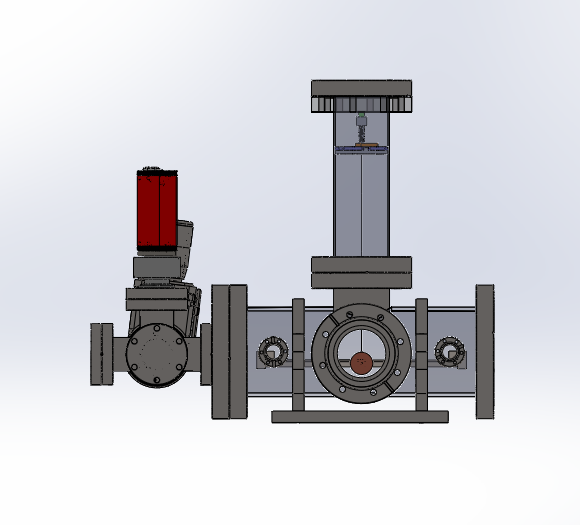
\includegraphics[scale=0.3]{\main/images/4 - methods and results/total_chamber.png}}
	\caption[Total chamber]{The system structure}
	\label{fig:Total chamber}
\end{figure}
\FloatBarrier
\par\noindent
The experiment is designed to minimize magnetic noises by avoiding capacitance and by choosing low magnetic permeability materials. Therefore, the torsional pendulum is placed inside a vacuum chamber, reducing Brownian motion, acoustic waves and friction. The vacuum chamber also reduces magnetic noise as a Faraday Cage. The vacuum chamber is placed inside seismic box, further reducing acoustic waves and magnetic noises from the environment. 

\par\noindent
The experiment system is designed to minimize the outgassing rate, by both choosing low outgassing materials and avoiding air pockets inside the devices. The design of torsional pendulum and vacuum chamber was carried out using Solid Works.

\subsection{Torsional pendulum design}
\begin{figure}[htbp]
	\centering
	\fbox{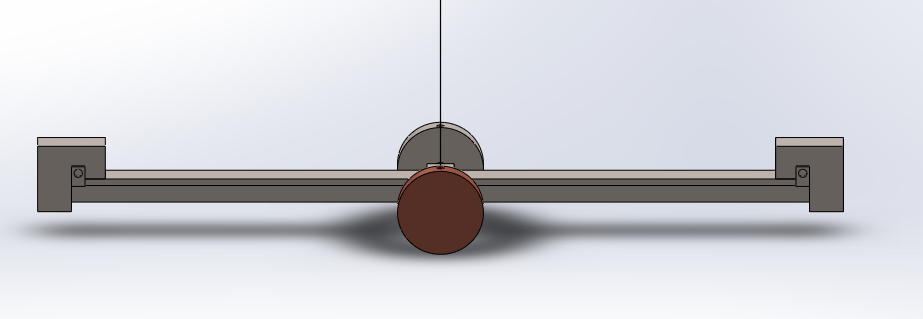
\includegraphics[scale=0.3]{\main/images/4 - methods and results/pendulum_front.png}}
	\caption[Torsional pendulum, front view]{Torsional pendulum, front view}
	\label{fig:pendulum front}
\end{figure}
\FloatBarrier
\subsubsection{Design constraints}
\par\noindent
The chosen pendulum dimensions are designed to balance the achievement of high angle sensitivity to field (large string torsion coefficient $\kappa$, eq.~\ref{eqn:gravitation_torque_equilibrium}) while maintaining high mass sensitivity to angle (longer oscillation time period $T$, eq.~\ref{eqn:theta average_2}). 
\par\noindent
For a torsional pendulum with length of $2l$, and two identical masses $m$ on the sides, the moment of inertia is:
\begin{equation}
I = 2ml^2     \label{eqn:moment_inertia_2}
\end{equation} 
As shown previously (eq.~\ref{eqn:undamped_omega}), for a torsional pendulum, the period is:
\begin{equation}
T = 2\pi\sqrt{\frac{I}{\kappa}}= 2\pi\sqrt{\frac{2ml^2}{\kappa}}   \label{eqn:undamped_motion_equation_4}
\end{equation}
Where $\kappa$ the string torsion coefficient is given by (eq.~\ref{eqn:torsion_coefficient_homogeneity}):
\begin{equation}
\kappa = \frac{G}{h} \frac{\pi d^4}{32}    \label{eqn:torsion_coefficient}
\end{equation}
\par\noindent
Longer string with smaller diameter results in a desired small string torsion coefficient $\kappa$. In order to achieve a string with as small a diameter as possible, tungsten string with high tensile strength was chosen. The high tensile strength allows a small diameter while overcoming suction forces when vacuum engine is working and holding the pendulum without tear. Tungsten is also vacuum compatible. 
\par\noindent
In order to minimize the magnetic noise in the measurements, the torsional pendulum was made out of stainless steel 316 (instead of stainless steel 304). Stainless steel 316 has a lower relative magnetic permeability $\mu_r$ \cite{SS316}.
\par\noindent
The experiment is constructed using a front mirror, where the angle displacement causes a mirror tilt. In order to minimize magnetic noise, the chosen mirror is made fully of metal (instead of coated glass). Having an oxygen-free copper (OFC) mirror, while not officially vacuum compatible, hopefully minimizes the vacuum outgassing.
\subsubsection{Technical information}
\begin{easylist}
& Tungsten string;
&& made of 99.95\% pure Tungsten
&& length $h$ of 249 mm
&& diameter $d$ of 0.08 mm
&& shear modulus $G$ of 130-160 [Gpa]\cite{tungsten}.
& Torsional beam;
&& made of Stainless steel 316
&& length $2l$ of 218 mm
% && width of 10 mm 
%& & weight of 90 gram 
&& identical side masses weight $m$ 20.5 gram
& Mirror;
&& made of oxygen-free copper (OFC), gold coated
&& diameter of 1 inch
\end{easylist}
\begin{easylist}
& results;
&& expected;
&&& $I = 0.487\cdot10^{-3}[kg\cdot m^2]$
&&& $\kappa = 2.1\cdot10^{-6}[\frac{N\cdot m}{rad}] - 2.6\cdot10^{-6} [\frac{N\cdot m}{rad}]$
&&& $T = 96[s] - 86 [s]$
&& experimental;
&&& $\kappa = 2.7\cdot10^{-6}[\frac{N\cdot m}{rad}]$
&&& $T = 84[s]$
\end{easylist}
\subsubsection{Design}
\par\noindent
The torsional pendulum angle tilt is measured using a mirror connected in front of the pendulum. The mirror is a part of an optical interferometer with which the mirror tilt could be determined.
\par\noindent
The pendulum center of mass needs to be adjusted, to avoid downward tilt of the mirror, due to earth gravity $g$. With a balanced pendulum the downward torque would be canceled out $\tau_y = 0$. The center of mass is adjusted using a balancing mass $m_1$ to the mirror's weight $m_2$ from behind:
\begin{equation}
\tau_y = 0 = m_1r_1g-m_2r_2g = m_1r_1g-m_2(w-r_1)g    \label{eqn:downward torque}
\end{equation}
\begin{equation}
\frac{m_1}{m_2} = \frac{w-r_1}{r_1}   \label{eqn:downward torque cancelled}
\end{equation}
\par\noindent
As shown in fig.~\ref{fig:pendulum top}, the balancing mass and the mirror are connected to the pendulum via spring $w$ from their center, and have a similar shape and weight. The spring enables accurate distance adjusting to prevent the downward tilt.
\begin{figure}[htbp]
	\centering
	\fbox{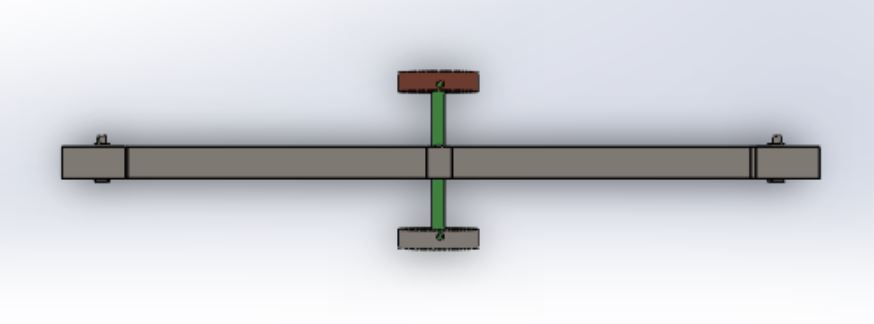
\includegraphics[scale=1.2]{\main/images/4 - methods and results/pendulum_top.JPG}}
	\caption[The torsional pendulum, top view]{The torsional pendulum, top view}
	\label{fig:pendulum top}
\end{figure}
\FloatBarrier 



\subsection{Vacuum chamber design}
\begin{figure}[htbp]
	\centering
	\fbox{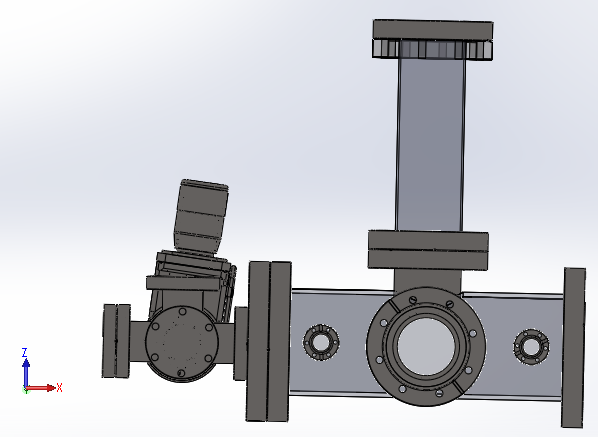
\includegraphics[scale=0.5]{\main/images/4 - methods and results/chamber_front.png}}
	\caption[Vacuum chamber, front view]{Vacuum chamber, front view}
	\label{fig:chamber front}
\end{figure}
\FloatBarrier

\par\noindent
The vacuum chamber is composed of two cylindrical tubes placed one over the other with three view ports in front. The chamber is connected to a vacuum engine and gauge.
\par\noindent
The vacuum chamber is bounded to the breadboard by an adjustable mount. The vacuum engine is connected to the chamber through a valve. Measurements are made when the valve is closed and the engine off, to prevent rotation noise.

\subsubsection{Chamber viewports}
\par\noindent
The central viewport is in front of the pendulum's mirror, to measure the tilt angle. Two small viewports on the sides of the chamber are used by the noise damping system (PID) to damp noises. 
\par\noindent
The view ports are for 550-1100 nm, with about 98$\%$ power transmittance in the range. The central viewport has a 68.3mm view diameter, and the distance from the mirror is 82 mm which gives a full field of view of about $39^0$ degrees (instead of $90^0$ at interferometry).

\subsubsection{Pendulum mount}
\begin{figure}[htbp]
	\centering
	\fbox{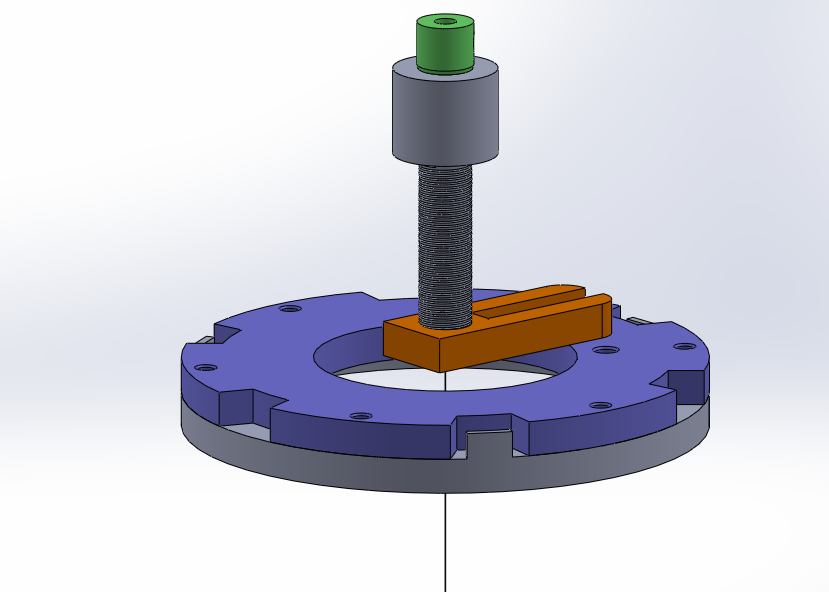
\includegraphics[scale=0.2]{\main/images/4 - methods and results/mount.png}}
	\caption[Pendulum mount]{Pendulum mount}
	\label{fig:mount}
\end{figure}
\FloatBarrier
\par\noindent
The upper tube of the chamber is soldered with a base to which a mount is connected. The pendulum string is held via the mount. The mount is adjustable, enabling the adjustment of the pendulum's string length, to place the pendulum in front of the viewports accurately. 

\section{Noise reduction}
\subsection{Pressure increase}
\par\noindent
Vacuum chambers are metallic chambers connected to a vacuum pump with pressure lower than the atmospheric pressure. The main limitations to vacuum quality maintenance are leakage $Q_L$ from the outside (eq.~\ref{eqn:leak rate}) through the chamber and outgassing $Q_{des}$ inside the chamber (eq.~\ref{eqn:desorption rate}), both increasing the pressure at a constant rate over time, and are overcome by having a constant pump rate $Q_P$ (the vacuum pump working constantly).   
\begin{equation}
Q_P = Q_L + Q_{des}  \label{eqn:vacuum_equilibrium}
\end{equation}
In this experiment, due to the relatively large size and unique shape of the measurement equipment, the vacuum chamber has a significant leak and outgassing rates. The pumping must be off during measurement, due to the measurement sensitivity, causing pressure increase over time.
\subsubsection{Minimized pressure increase}
\par\noindent
In order to minimize the pressure increase, the vacuum chamber was built using CF style vacuum components, designed for ultra high vacuum, minimizing the leak rate. ALSO, the vacuum chamber and measurement system were baked-out to reduce outgassing, using resistive wire. The bake-out was carried out for a week at about $110 C^0$ achieving stable vacuum of about $2\cdot 10^{−4} [Torr]$ after cooling down.
\par\noindent
\subsection{Pressure affect}
\par\noindent
As demonstrated previously (eq.~\ref{eqn:heat conduction 2},eq.~\ref{eqn:total_kinetic}, eq.~\ref{eqn:acoustic_intensity}, eq.~\ref{eqn:drag force}), Brownian motion from the environment, thermal coupling, acoustic waves and friction are pressure dependent and are considerably reduced by maintaining low pressure.
\par\noindent

\subsection{Faraday cage}
\par\noindent
The Faraday cage is a cage made by continuous covering of a conductive material used to block external electromagnetic fields. The external electrical fields cause an electric charge distribution in the conductive cage without passing inside. Electric current decays exponentially with depth through the material. The material skin depth $\delta$ defines the magnetic field's penetration depth, given by:
\begin{equation}
\delta = \sqrt{\frac{2\rho}{(2\pi f)(\mu)} }    \label{eqn:skin depth}
\end{equation}
Where $\rho$ is the material electric resistivity, $\mu$ the magnetic permeability and $f$ is the frequency of the magnetic field.
\subsubsection{Seismic box and vacuum chamber}
\par\noindent
The measurement system is placed inside a seismic box which is a Faraday cage with 76 mm thickness, blocking magnetic fields with $f \ge 30 [Hz]$ from the environment. The seismic box is both reducing acoustic waves and magnetic noises from the environment.
\par\noindent
The vacuum chamber is a second cage blocking magnetic noise from the electronic system placed inside the seismic box. Vacuum chambers are made out of approximately 3 mm thick stainless steel, blocking magnetic fields with $f\ge 20 [KHz]$ while reducing magnetic noises from lower frequency fields.


\section{Modulated light source}
In front of each of the viewports on the sides of the chamber there is a controlled LED light source, coupled to a side mass of the pendulum. The light sources are controlled by a PID algorithm through a computer and are used to generate torques in real time to actively damp the pendulum noises in real time.
\subsection{Radiation pressure force}
The difference between two torques from both ends of the torsional pendulum add a small external net torque:
\begin{equation}
\tau = l\cdot F_1 \cdot cos\alpha_1 - l\cdot F_2 \cdot cos\alpha_2  \label{eqn:radiation torque}
\end{equation}
Where $\alpha$ is the force incident angle compared to the pendulum surface. Light source with a given flux causes a radiation-pressure force (eq.~\ref{eqn:radiation_force_power}). The radiation-pressure net torque assuming that both light fields have the same coupling efficiency and are very close to being perpendicular to surface, causing both incidence angles to be negligible:  
\begin{equation}
\tau \approx l(F_1 - F_2) \approx \frac{2l\eta}{{c}} (\Theta_1 -\Theta_2) \label{eqn:radiation net torque}
\end{equation}
\par\noindent
\subsection{Arduino microcontroller}
Arduino is an open-source microcontroller board used for building inexpensive digital circuits, containing microprocessor, controller and serial communication interface. The Arduino Mega 2560, is based on the ATmega2560 8-bit controller, and equipped with a $16 [MHz]$ crystal oscillator (clock) and 15 PWM outputs pins. The Arduino Mega's output is a digital output $V_d = 5[V]$ without a digital-to-analog converter (DAC), but it can simulate analog output using Pulse Width Modulation (PWM). 
\subsubsection{Pulse Width Modulation}
\begin{figure}[htbp]
	\centering
	\fbox{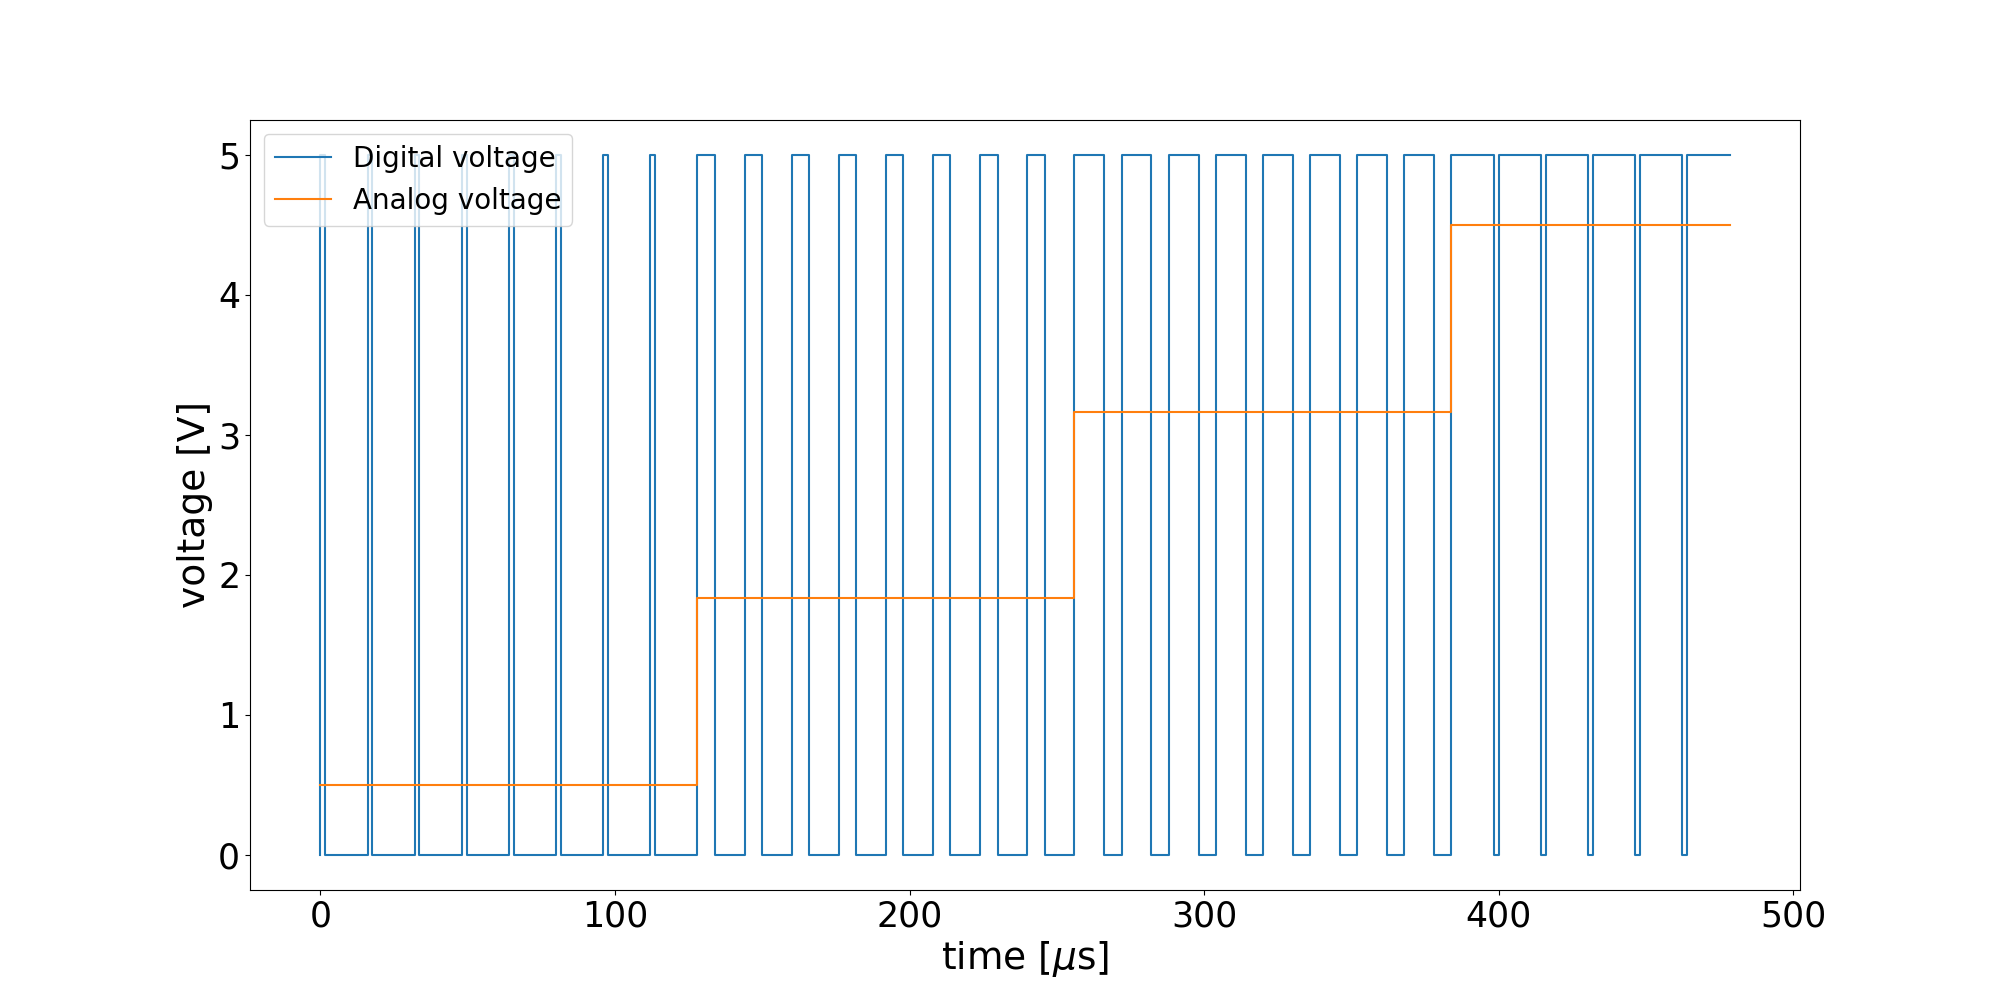
\includegraphics[scale=0.5]{\main/images/4 - methods and results/duty_cycle.png}}
	\caption[The PWM analog voltage]{The PWM analog voltage}
	\label{fig:duty_cycle}
\end{figure}
\FloatBarrier
\par\noindent
As shown in fig.~\ref{fig:duty_cycle}, the controller switches the output signal fast between the digital output on and off, generating a square wave with period $T$. Pulse width ($PW$) is the time duration in which the signal is on. With the clock, the controller is able to modulate $PW$, changing the ratio of time signal is on compared to off, which is the duty cycle $D$:
\begin{equation}
D(t) = \frac{PW(t)}{T}\cdot 100  \label{eqn:duty cycle}
\end{equation}
The duty cycle varies between 0 to 100\%, with resolution limited by the controller. The Arduino is modulating the duty cycle, resulting in modulation of the The analog voltage (the average voltage) $V_a$ given by: 
\begin{equation}
V_a(t) = \frac{ PW(t)\cdot V_d}{ T}  = \frac{V_d}{100}\cdot D(t)  = \frac{5}{100}\cdot D(t)  \label{eqn:pwm voltage}
\end{equation}
Since the Arduino clock is connected to all PWM pins, they are all in sync. When all PWM pins have the same duty cycle, they all have the same voltage, frequency and phase. Even though the pins output vary in time, they are constant voltage supplies compare to each other, allowing to connect $N$ pins in parallel and increase the output current $I_{total}$ given by: 
\begin{equation}
I_{total} = N\cdot I   \label{eqn:pwm current}
\end{equation}
The clock is having about 120 full periods of the square wave before changing to a new duty cycle value, limiting the voltage modulation frequency. Also, in order to be able to change the duty cycle, the clock frequency is limited by the controller bit-rate. The PWM frequency is given by:
\begin{equation}
f_{PWM} = \frac{1 }{120T}= \frac{1 }{120 \frac{8-bit }{16MHz}}  \approx 500[Hz]	    \label{eqn:pwm frequency}
\end{equation}
\subsection{Light emitting diode (LED)}
The light emitting diode (LED) is a semiconductor based light source with high power, and a long lifetime. Forward voltage is applied to a p-n junction, causing electron injection and recombination with holes. The recombination is releasing energy in form of spontaneous emission photons (incoherent light). Due to the electrons life time before recombination, the LED could be modulated up to $100MHz$.
\par\noindent
The LED opening angle (FOV) varies between 45 to 120 degrees, and the emitted light is incoherent in width meaning it's hard to focus it to a point (not diffraction limited) and incoherent in length causing wide band spectrum. The LED current $I$ is defined by the Shockley diode equation for p-n junctions:
\begin{equation}
I  = I_s (e^{V_l\cdot \frac{e}{n k_B T} }-1) = I_s (e^{\frac{V_d}{n V_T} } -1) \overset{V_d>>V_T}{\approx} I_s e^{\frac{V_d}{n V_T} }   \label{eqn:led current}
\end{equation}
Where $I_s$ is the saturation current of the diode, $V_l$ is the LED forward voltage, $n$ is the led emission coefficient, $e$ is the electron charge, and $V_T$ is the thermal voltage. The LED forward voltage is given by:
\begin{equation}
V_l \approx n V_T ln10 log_{10} (\frac{I}{I_s}) \label{eqn:led voltage}
\end{equation}
\subsection{LED setup}
Since the forward voltage $V_l$ varies as the logarithm of the current, it varies slowly, being approximately constant over wide current range, resulting with large changes in the LED current due to small changes in the circuit supply voltage $V$. Driving circuit composed of resistor $R$ in series with the LED stabilizes the current, given by:
\begin{equation}
I =\frac{V-V_l}{R} \label{eqn:led circuit}
\end{equation}
The circuit is composed of a blue LED with $V_l\approx 4.5V$, supply voltage with 6 parallel PWM Arduino pins (eq.~\ref{eqn:pwm current}, eq.~\ref{eqn:pwm voltage}) and resistor $R = 200\Omega$, the LED radiant flux $[W]$ is given by:
\begin{equation}
\Theta(t) = I_{total}\cdot V_l = NI\cdot V_l = N V_l \frac{V-V_l}{R}\cdot  =N V_l\frac{\frac{5}{100}\cdot D(t)-V_l}{R} \approx N V_l\frac{\frac{5}{100}\cdot D(t)}{R} = 0.007\cdot D(t)\label{eqn:led power}
\end{equation}
\par\noindent
In order to overcome the led uncoherent profile and large FOV, the light is coupled to a light guide, a pipe made of thin filaments causing internal reflections used  to illuminate small areas, regardless of the spectral characteristics of the light source. Light guide mainly depend on the entrance and exit cross section and length, making it ideal to overcome focusing problems. 
\par\noindent
Due to coupling efficiency and size difference between the output beam from the lightguide and the pendulum sides, the efficiency of flux hitting the pendulum is estimated to be $\eta = 0.7$ and the torque is given by:
\begin{equation}
\tau(t)  =\frac{2l\eta}{{c}} (\Theta_1(t) -\Theta_2(t)) = 3.56^{-12}(D_1(t) -D_2(t)) 
\label{eqn:led tourqe}
\end{equation}
\par\noindent
The LED power could be approximated by linear approximation of the Arduino duty cycle $D(t)$, which varies between 0 to 100\% with 8bit resolution, generating torques up to $\tau = 7\cdot10^-{10} [N\cdot m]$ with modulation steps of $\Delta\tau = 1.4\cdot10^-{12} [N\cdot m]$. As shown in eq.~\ref{eqn:pwm frequency}), the LED could be modulated up to $500[Hz]$ resulting with fast modulated external force for the PID algorithm. Also, since the led power could be approximated using linear approximation, it allows to control the approximated power output by changing the PID gain values.  









\subsection{Active noise damping}
\par\noindent
After the desired vacuum is achieved, the vacuum engine is disconnected using the valve and turned off, and the seismic box is closed. After approximately eight hours the pendulum oscillations damp down to a level which could be affected by the weak force caused by radiation pressure.


\par\noindent
ThePID is damping the noises, and after they are damped the measurement begins.

















\section{Proportional–Integral–Derivative (PID)}
\subsection{Damped oscillator}
PID controller can continuously calculates error value of an oscillator, to damp it to zero. If the defined set point is set to zero, the error is the measured process variable. The PID acts as friction, gradually working when the oscillations are at the maximum speed to slow them down, and remove the torque energy.
\begin{equation}
e(t) = \theta(t) = \theta   \label{eqn:error}
\end{equation}
\begin{equation}
\tau_{PID} = -\gamma\cdot\dot{\theta}   \label{eqn:friction_torque_pid}
\end{equation}
The system is a damped oscillator, with an external force correction, which inserts torque to the oscillator.
\begin{equation}
\kappa\cdot\theta - \gamma\cdot\dot{\theta}  + I\cdot\ddot{\theta} = 0   \label{eqn:damped_pid_motion_equation}
\end{equation}
\begin{equation}
\gamma\dot{\theta}  = LF   \label{eqn:damped_pid_motion_equation_1}
\end{equation}
\begin{equation}
\dot{\theta} = \omega_0\theta_{max}sin(\omega_0 t +\phi)    \label{eqn:undamped_motion_equation_1}
\end{equation}
\begin{equation}
\dot{\theta}_{max} = \omega_0\theta_{max} = \theta_{max}\cdot\frac{2\pi}{T}    \label{eqn:undamped_motion_equation_3}
\end{equation}
\begin{equation}
\gamma  = \frac{LF_{max}}{\dot{\theta}_{max}} =\frac{LF_{max}T}{\theta_{max}2\pi}    \label{eqn:damped_pid_motion_equation_2}
\end{equation}
\begin{equation}
\tau =  \frac{2I}{\gamma}  \label{eqn:damping_time_pid}
\end{equation}
The PID damping $\gamma$ and damping time $\tau$ depends on the initial oscillations angle. If the angle is too large compare to the inserted force, the system is extremely underdamped and the PID affect is negligible. The damping time would be infinite and the system would keep on oscillating.

\subsection{Control stability}
Using PID control does not guarantee optimal control or stability. The control system is aiming to achieve critical damping of the process. Well tuned control would a reach the desired set point fast and accurate, and also apply over time the necessary corrections to resist external forces trying to move variable from the set point.
\par\noindent
The controller response is its response to error. How much does the system overshoots a setpoint and the system oscillations. When controller gains are too high, instead of critical damping there is overdamping causing overshoot, due to the high gain the overshoot response overshoots to the other side, causing the system to be driven.










\section{Modulated CW laser}


\section{Modulated LED}

















\section{pid operate (algorithm)}
\section{laser +aom +amp}
\doublespacing



\section{Overshoot}
Overshoot is when output signal or function exceeds the target value. The response signal is not accurate compare to target. In control theory there are two wanted conflicting properties; an accurate response (small overshoot), and small risetime (fast response). 
\par\noindent
Overshoot is usually measured in percentage overshoot (PO). For second order systems, such as damped oscillators PO is a function of the damping ratio $\xi$. 


\begin{equation}
PO = 100\cdot e ^{\frac{-\xi\pi}{\sqrt{1-\xi^2}}} = \frac{output-target}{target}   \label{eqn:percentage_overshoot}
\end{equation}
 
\section{Accuracy}

\subsection{Laser}


The laser is a high power coherent light source based on stimulated emission with narrow spectrum. Inside a cavity Electron is excited to a higher energy level, and forced by photon with the correct wavelength to be absorbed emitting coherent photon. The coherence allows focusing beam to a tight spot, and being collimated over long distances. Continuous wave (CW) laser are lasing constant output power over time.



\par\noindent
Usually the power output is stable but has oscillations due to having several longitudinal modes causing nano second scale oscillations, output power is steady when averaged over longer periods. Also, over long periods of time lasers have slight power oscillations due to temperature changes in the environment.
%The laser diode cavity face is rectangular, because of fabrication constraints. The rectangular face is causing cylindrical aberration, which   

\subsection{Acousto optic modulator}
Acousto Optic Modulator (AOM), uses the acousto-optic effect to diffract and shift the frequency of light using RF waves. An oscillating electric signal drives a piezoelectric transducer to vibrate causing RF waves, the transducer attached to a material. This causes sound waves in the material, and periodic index modulation causing a Bragg grating. Incoming light scatters off the grating and due to Bragg diffraction comes at Bragg angle.
\begin{equation}
\theta_b = sin(\theta_b)\approx \frac{\lambda}{2n\Lambda} \label{eqn:aom angle}
\end{equation} 
$\Lambda$ is the RF wavelength, $\lambda$ is the light source wavelength. 
\par\noindent
Since all parameters constant, modulation angle is constant, and possible modulation speed is nano seconds. Giving a stable fast modulation method for CW laser.

\end{document}